\section{Durchführung}
\label{sec:Durchführung}
Eine schematische Darstellung des Versuchsaufbaus ist in \autoref{fig:Aufbau} zu finden.
\begin{figure}[H]
  \centering
  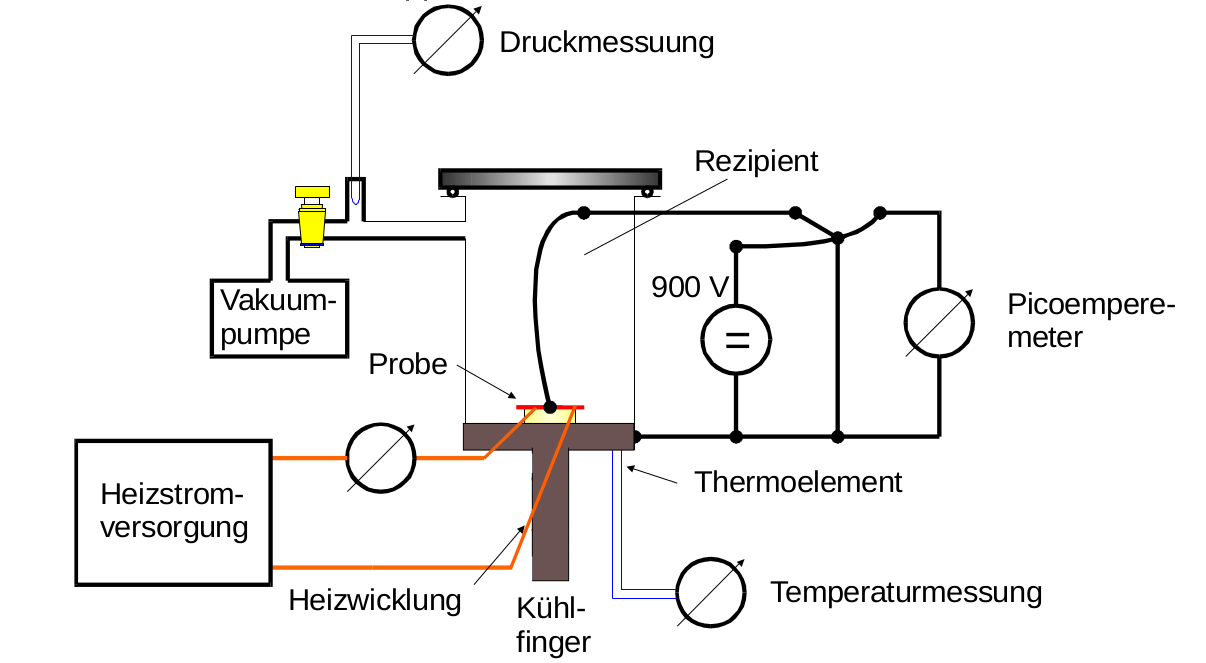
\includegraphics[width=0.6\textwidth]{pics/Aufbau.png}
  \caption{Schematische Darstellung des Versuchsaufbaus \cite{Anleitung}.}
  \label{fig:Aufbau}
\end{figure}
Die mit Strontium dotierte Kaliumbromid Probe befindet sich in einem Plattenkondensator,
welcher sich wiederum in einem, mit einer Vakuumpumpe auf ca. $10^{-2}\,$ Torr evakuiertem, Rezipienten befindet.
Dies wird gemacht, um die Umgebung der Probe von $\text{H}_2\text{O}$-Molekülen zu befreien, da
diese auch Dipole besitzen, welche die Messung verfälschen würden.
Des weiteren sind Heizstromversorgung, ein Gleichspannungs-Netzgerät sowie ein Thermoelemet und
ein empfindliches Amperemeter angeschlossen.\\
\\Die Probe wird zunächst auf eine Temperatur von ca. $50\,$°C erhitzt. Danach wird
das Netzgerät mit einer Spannung von $950\,$V eingeschaltet und die Probe für $900\,$s
im Feld gelassen. Nach dieser Polarisationszeit wird die Probe, durch das Eintauchen des Kühlfingers
in flüssigen Stickstoff, auf ca. $-70\,$°C abgekühlt. Der Plattenkondensator wird
kurzgeschlossen und das Picoamperemeter angeschlossen.
Nach der Messung des Offsets des Amperemeter wird mit der Messung begonnen.
Mit einer konstanten Heizrate von $1,5\,$°C pro Minute wird die Probe erwärmt und
in einem Abstand von jeweils einer Minute wird sowohl die Temperatur als auch der
gemessene Relaxationsstrom gemessen.\\
In einer zweiten Messreihe wird das selbe Verfahren noch einmal durchgeführt, jedoch mit
einer Heizrate von $2\,$°C pro Minute.
